\chapter*{Presupuesto}
\addcontentsline{toc}{chapter}{Presupuesto}
\markboth{PRESUPUESTO}{PRESUPUESTO}

A continuación se hace una estimación de los costes que conlleva la realización de este \gls{PFC}.

Para ello, en primer lugar se ha confeccionado un calendario con las tareas realizadas. Se ha asumido para la realización de este calendario que:

\begin{enumerate}
  \item Los trabajos dan comienzo el día 2 de enero de 2017.
  \item La dedicación de la persona que desarrolla el trabajo es del 100\% distribuida en una jornada laboral de 8 a 12 y de 13 a 17 horas.
  \item La ausencia de días festivos. Solo se tienen en cuenta los fines de semana.
  \item Se da una situación ideal sin interrupciones de ningún tipo de por medio, pudiendo realizar los trabajos uno detrás de otro.
\end{enumerate}

Se considera también que la persona encargada de realizar estos trabajos tiene el nivel de ingeniero junior. La tarifa que se aplica a esta persona es de 35 euros la hora sin IVA.

En cuanto a la infraestructura, deberá estar disponible durante los 6 meses posteriores al inicio del proyecto. Este coste también será tenido en cuenta en el presupuesto.

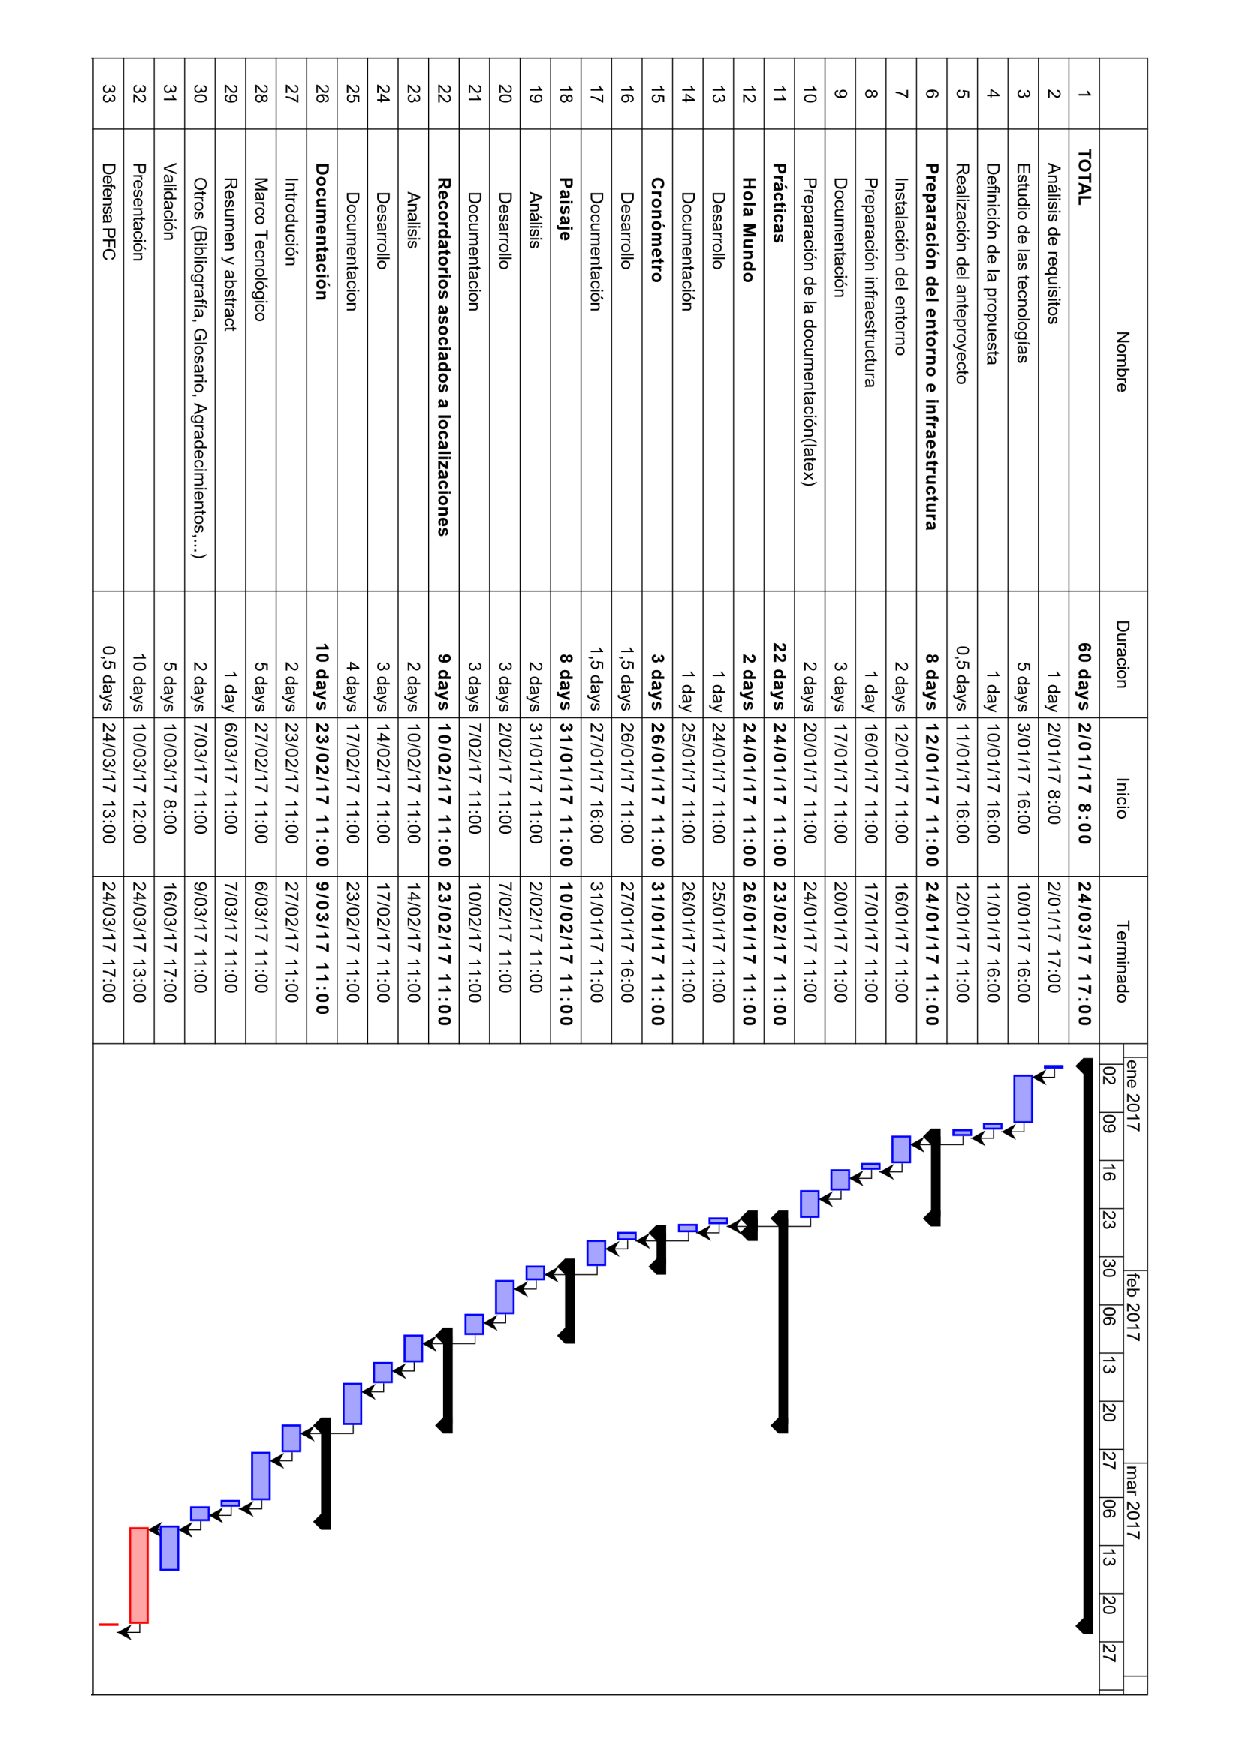
\includepdf[pages=1,scale=0.85,offset=30 -10,pagecommand={\pagestyle{fancy}}]{Presupuesto/calendar_1.pdf}
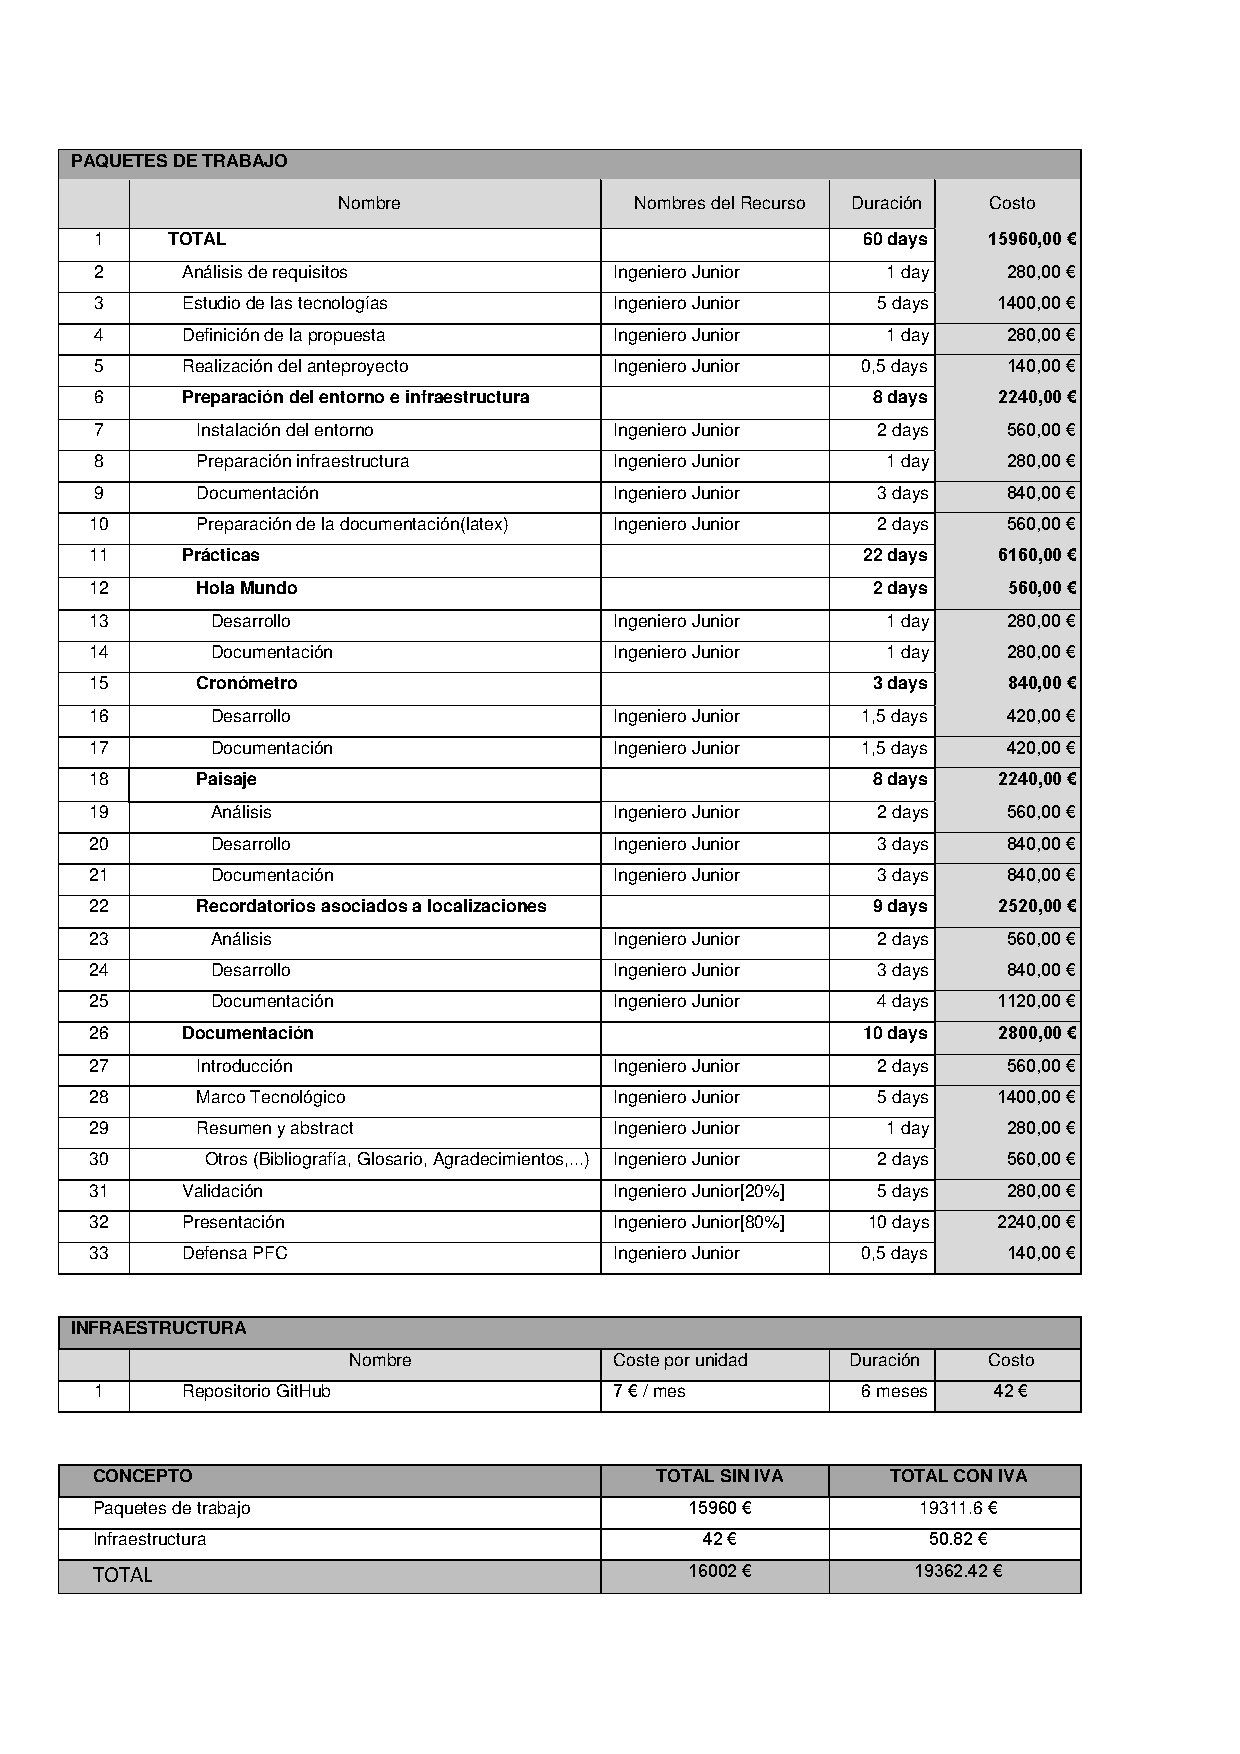
\includepdf[pages=1,scale=0.85,offset=50 20,pagecommand={\pagestyle{fancy}}]{Presupuesto/cost_1.pdf}
